\documentclass[12pt,a4paper]{article}
\usepackage{times}
\usepackage{durhampaper}
\usepackage{harvard}
\usepackage{algorithm}
\usepackage{algpseudocode}
\usepackage{array}
\usepackage{graphicx}
\graphicspath{ {images/} }

\citationmode{abbr}
\bibliographystyle{agsm}

\title{Formatting Template for the Final Paper}
\author{Edward Hockedy}
\student{Edward Hockedy}
\supervisor{Dr. Magnus Bordewich}
\degree{MSc Computer Science}

\date{}

\begin{document}

\maketitle

\begin{abstract}
These instructions give you guidelines for preparing the design paper.  DO NOT change any settings, such as margins and font sizes.  Just use this as a template and modify the contents into your design paper.  Do not cite references in the abstract.

The abstract must be a Structured Abstract with the headings {\bf Context/Background}, {\bf Aims}, {\bf Method}, and {\bf Proposed Solution}.  This section should not be no longer than a page, and having no more than two or three sentences under each heading is advised.
\end{abstract}

\begin{keywords}
Put a few keywords here.
\end{keywords}

\section{Introduction}
Robotics is a rapidly advancing field with important applications in a wide range of fields. The primary aim of a robot in most cases is to emulate and improve upon actions carried out by a human, or enable the completion of a task a human is incapable of completing. Examples of such uses include job automation, social care, dangerous environment exploration, entertainment, and many more. One of the most difficult aspects of creating a working robot is programming how it will move and behave. In some very specific cases it is sufficient to explicitly tell the robot exactly what it must do complete the task, and how to do it. In general though, it is preferred to allow the robot to discover itself the best actions to take are. This has two main benefits. Firstly, it does not require a full description of what the robot must do to complete the task. Fully explaining a task and every possability that may arise is difficult of all but the simplest tasks. As such, it is better to have the robot learn how to coplete the task in general, such that when faced with a slight variation or new scenario it can adapt of change it behaviour to what it thinks is the best way to tackle the task as opposed to just following what it always does. Secondly, a human may not describe the most efficient way to complete a task. By havng the robot discover or observe a task by itself, it may work out a more efficient way to complete a task than previously thought. 

This project partly looks at different methods of enabling a robot to learn to complete a task. The task examined in this case is balancing a ball on a tray in two dimensions. The robot can observe the ball and carry out one of two actions, either tilt clockwise or anticlockwise, in an attempt to keep the ball in the centre and with a low velocity. 

The methods studied fall into two categories - supervised learning and reinforcement learning. Supervised learning provides examples of actions taken given a scenario. From this, the robot learns which actions are good to take in each situation, and can interpolate based on the learnt model what to do in an unseen state. This is equivalent to the robot observing a human complete the task. It does not require every possible state to be shown to it, just enough so that it can get a general idea of what behaviour leads to what outcome. In this project, the behaviour was captured using a neural network, and the data generated using a simulation of a tray and ball that could be controlled by a user. Reinforcement learning is where the robot is told what a good state to be in is, and by trying out different actions the robot receives a reward or punishment dependent on the quality of the state it transitions to. It requires the robot to try out many actions in training. During this training the robot updates its idea of what a good action to take in each state is, and slowly learns the behaviour to maximise its reward. In this project, the method used is Q-learning with a Q-table. 

Another aspect of this project is the use of simulation in training the robot. Since both reinforcement learning and supervised learning require the robot to repeately trial or perform a task, it can be very time consuming to carry out the task in real time on the actual robot, or access to the robot may not be possible. As such, a simulation of the tray and ball environment has been created and used. The purpose of this is to allow for much faster reinforcement learning training or supervised learning data generation. The simulation is not a perfect recreation of how the tray and ball behave in real life, so this project also explores the suitability of using a simulation to approximate real world behaviour, and assessing how well the learnt behaviour transfers from the simulation to the robot. 

\section{Related Work}


\section{Design}

\subsection{The Task}
The task chosen for the robot to learn to perform was to balance a ball on a tray. The ball can move in one dimension, either to the left or the right. The goal for the robot is to keep the ball stable - in the middle of the tray with the velocity low. This is done by performing one of a number of three actions, tilt the tray clockwise, tilt the tray anticlockwise, or keep the tray at the angle it currently is. At each step of the task, the robot can observe information about the environment. This information comprises of the horizontal position of the ball relative to the robot, with the origin at the centre, the horizontal velocity of the ball, and the angle the tray is currently tilted at. These pieces of information are continuous, and as such it is infeasible to describe the required action for all possible states. To get around this, these values are mapped to a discrete division that encompasses the value and similar values. For example, the position of the ball may be grouped into one of 10 possible positions on the tray. The combination of these three bits of information of position, velocity and angle, makes up the current state of the environment. The task is to have the robot learn what the best action to take given any state.

This task was chosen for a few reasons. Firstly, it is simple enough to be acheivable by a robot given the chosen learning techniques. The number of states is fairly small, but big enough that it is hard to outright describe what to do in every scenario. Following from that, the system is complex enough to be difficult to describe without mathematically modelling the whole system, but simple enough that the leant model can interpolate to unseen scenarios. The task is also one acheivable by humans in a basic sense of just standing still, but becomes difficult when extra tasks are included such as walking forward. As such it is hoped that the robot could surpass human performance if it learns well enough. Finally, the task has obvious real world applications. Whilst the level of performance acheived in this project is insufficient to have much real world impact, a high level implementation of this behaviour could be used to carry object accross a room, perhaps to an immobile patient, or to carry a person out of a dangerous environment.

\subsection{The Robot}
The robot used is the Nao from SoftBank robotics. It is a humanoid robot standing at 58 cm tall. It is fully programmable using the Python API and allows for full control over the angles and position of joints. It has built in vision capabilties that utilise the cameras located on its head. For the setup of this task, the Nao robot is standing with its arms stretched out. It grabs on to a cardboard tray  and holds it close to flat infront of it. There is a small track that the ball sits in to prevent it from falling off the back or front of the tray, and two side buffers to prevent it from falling off the sides. The robot has built in functionality to track a red ball which is the method used in this project. At any time the position in 3D space of the ball can be calculated by the robot. The velocity can then be obtained by observing the changein position over a small time period. The tray is tilted by the robot moving it arms. To determine the range of possible angles the robot can move between, the robots arms were positioned by hand and the angles of the upper body joints were recorded. They were then manipulated so that the same angle could be recreate but in the opposite direction. The robot can then interpolate any angle between the maximum and minimum by taking a porportion of the maximum tilt and minimun tilt and adding the angles together.

\subsection{Simulation}
As previously mentioned in section I, the simulation helps to greatly speed up the training process. This allows for much more experimentation to find the best parameters for each method. The simulated environment is two-dimensional and comprises of a ball that rests on a tray that can tilt. The tray has barriers at either end to stop the ball from rolling off the ends of the tray. The tray can be tilted up to a maximum angle in each direction. This simulation was built using the Pymunk physics engine. At each stage of the simulation the position and velocity of the ball can be directly read, as well as the angle of the tray.  
\subsection{Reinforcement Learning Approach}
As described in \cite{rl_survey}, "Reinforcement learning is the problem faced by an agent that must learn behavior through trial-and-error interactions with a dynamic environment". What this means is that the agent (the robot/simulation) must learn how best to balance the ball by repeatedly trying different actions to try to get the bal in to a good state. Over time the agent will try different actions to what it currently thinks is the optimal action to take. By doing this, it prevents the agent from learning the first thing it finds successful, as there may be an even better action that it is yet to try. The method of reinforcement learning used in this project is Q-learning. Q-learning is a model-free reinforcement learning technique. Being model-free means there is no pre-learnt model that the actions are based off, it relies fully on the trial-and-error experiences for learning actions. Over time, the agent learns the best action to take when in each state. This information is stored in a Q-matrix. This is a large matrix for an entry for each possible state the ball can exist in. For each cell there is an array of length equal to the number of possible actions the agent can take. A value is stored for each action, with the value representing how good of an action it is given the current state. The process of learning works by the agent first observing the state it is in. It then looks at the Q-matrix and decides what the best action it can take is - the one with the greatest value. It carries out the action and observes the new state it ends up in. It also receives a reward dependent on how good this new state is. The value for the action taken from the old state is then updated using the exising value, the reward, and the value of the best possible action to take given the new state. The intuition behind using the best value of the new state is that Q-learning assumes the agent is follwing an optimal policy - the best possible chain of transitions between states, taking the optimal action each time. This is of course not the case during training, but over time it should converge to this. The update policy can be formalised as:
\[Q(s_t, a_t) = (1 - \alpha) \cdot Q(s_t, a_t) + \alpha\cdot(r_t + \gamma\cdot max Q(s_{t+1}, a)) \]
$s_t$ is the state at time t \\
$a_t$ is the action taken at time t \\
$r_t$ is the reward observed by taking $a_t$ from $s_t$\\
$\alpha$ is the learn rate. The higher this is the higher the updated value takes into account the reward and future state information compared with the existing value\\
$\gamma$ is the discount factor. The higher this is, the more important future values are taken to be. A small value only looks at the immediate future of the next few transitions\\

For the implementation of Q-learning in this project, the reward was determined in two ways. The first was with a very specific reward, based on what a human would intuitively think is the best action to take at each step. It used both the current state information and previous state information. The reward is decided based on the following criteria:
\begin{algorithm}[H]
	\caption{Calculate reward using very specific criteria}
	\label{ql_specific}
	\begin{algorithmic}[1]
		\State $reward = 0$
		\If {$current\_velocity > 0$ \textbf{AND} $current\_angle > previous\_angle$}
			\State $reward = 1 - |\frac{current\_position}{tray\_width}|$
		\ElsIf {$current\_velocity < 0$ \textbf{AND} $current\_angle < previous\_angle$}
			\State $reward = 1 - |\frac{current\_position}{tray\_width}|$
		\ElsIf {$|current\_velocity| < max\_velocity*0.01$ \textbf{AND} $|current\_position| < |previous\_position|$}
			\State $reward = 1 - |\frac{current\_position}{tray\_width}|$
		\Else 
			\State $reward = -1 * (1 -|\frac{current\_position}{tray\_width}|)$
		\EndIf
	\end{algorithmic}
\end{algorithm}
Algorithm 1 gives a positive reward if the ball has a positive velocity (left to right) and the tray has moved anticlockwise, effectively slowing it down, and vice-versa on line 4. It also gives a positive reward if the ball is at the very low speed of 1\% of the maximum speed, and moving towards the centre of the tray. Since the tray is centered on 0, the magnitude of the position determines how close to the centre the ball is, with a smaller magnitude meaning the ball is closer. If none of these cases are matched, then a negative reward is given. In each case of the reward, the size is determined by how far the ball is to the centre, with a bigger reward being given if the ball is closer to the centre.

The second reward scheme is much simpler, using only the current state information to specify the states that deserve a good reward, with everything else getting a negative reward. The reward scheme is outlines in algorithm 2.

\begin{algorithm}[H]
	\caption{Calculate reward using very general criteria}
	\label{ql_general}
	\begin{algorithmic}[1]
		\State $reward = 0$
		\State $n_1, n_2 = n$
		\If {$central\_p\_segment - n_1 < p\_segment < central\_p\_segment + n_1$ 
			\textbf{AND}
			 $central\_v\_segment - n_2 < v\_segment < central\_v\_segment + n_2$}
			\State $reward = 1$
		\Else 
			\State $reward = -1$
		\EndIf
	\end{algorithmic}
\end{algorithm}
Algorithm 2 gives a positive reward if the ball is in one of the segments determined to be good. The middle segment for position is the one closest to the centre. The middle segment for velocity is the one closest to 0. As such, the ideal state is to be in both of those segment. $n_1$ and $n_2$ extend the range of the desired segments as required, with $n$ being an arbitrary integer.

The training begins with the ball dropped into a random position and the tray at a random angle. At each step the agent chooses the action it thinks is the best for the given state. No prior knowledge is given for Q-learning, so all table values are 0. In order to assign values, at the start there is a very high probability of taking a random action. This probability is known as the explore rate. This allows the agent to slowly build up some scores for taking actions at different states. Over time the Q-matrix fills up and the values should start to converge. The explore rate decreases over time to allow the agent to start taking the best actions. Most states will have been sampled after enough time, so exploration is not needed. The Q-matrix should end up with the states all suitably sampled, and the rewards/punishments should have propagated through via the update function such that a distribution of state quality exists through the matrix. 
\subsection{Supervised Learning Approach}
The first step in the supervised learning approach was to generate the training data. To do this the simulation was altered so that it could be moved by user input. A ball would be dropped onto the tray at a random angle, and a user could press keys to rotate the tray one angle segment clockwise or anticlockwise, depending on what was required to keep the ball balanced. At each key press, the state and action taken was recorded. This was repeated over many iterations to build up a reasonably sized data set that covered many situations. 
The model used to learn the pattern is a neural network. A neural network is a way to theoretically simulate any function, by combining many simple, linearly-seperable functions known as neurons. The neurons exist in layers with one input layer and one output layer. Between the layers exists weights from each neuron to each neuron in the next layer. The network is trained by passing through the input data. Each neuron receives some input from the previous layer, maps the combination of input values to an output value depending on its function, then outputs a value that goes to the next layer. Once the input data has passed through the network, the output from the network is compared with the actual output from the training data. The difference is calculated and that error is used to refine the weights between the neurons. As more data is passed through, the network gets refined and begins to learn which inputs lead to which outputs.

For this project, then input value is the state of position segment, velocity segment and angle segment. The output is one of the three possible actions, encoded with one-hot encoding. 

MAYBE PUT THE FOLLOWING LATER DOWN
This approach differs from the reinforcement learning approach because the agent is outright told what is a good action to take in a given state. This is not necessarily bad for machine learning, and works well because the ball balancing task is simple. However, in general it might not be suitable for a more complex task, since it is almost impossible to fully describe eactly how an agent should behave. Another downside to this technique is that it requires generation of training data from human input. This means the agent can only really do as well as the human can. 
This technique is useful because it allows for interpolation between states, which means it deals well with unfeen circumstances. The neural network always gives an output no matter what, and assuming it has seen some somewhat similar cases it should give a decent output. In contrast, the Q-matrix may have some blank cells that have never been expored before, meaning there is no way to infer what a good action to take would be. Training time and data size are also an advantage with the neural network. The Q-matrix has to store data for every single state, and since a state is a 3-dimensional vector, the state space grows fast, which means training takes a long time too. The neural network stays the same size however, and whilst its size can vary, it will not be close to the size of the Q-matrix. The training data may be quite large, but once the model is trained it is not required. 

\subsection{From Simulation To Robot}
Once trained, the Q-matrix and neural network could both be used in conjunction with the robot. With the tray held out and the ball place on, the robot will track the ball, moving its head as it moves, and take actions based on what the neural network or Q-matrix decides is best. There were a few difficulties that arose with using the robot, as well as some parameters that needed to be chosen. The biggest issue was that the arms of the robot overheated quickly. For safety reasons, this means the stiffness in the overheated joint goes to zero meaning the joint cannot be moved. This usually happend about ten minutes after having the robot move its arms freqeuently. Whilst this was not a huge issue in the long run because the focus was to do all training in simulation, any training or data collection that happened on the robot becaus edifficult and time consuming when waiting for the robot to cool down. A good work around was to have two robot on the go, and use one whilst the other cooled down. This issue very much highlights the usefulness of simulation in robot movement training.

Another issue was the accuracy of the ball tracking. The built in tracker could detect the position of the ball upon a function call. In order to have a continuous update of ball information, the tracking function was continuously called by a thread running in the background. An issue arose when choosing the frequency of updating the ball information however. Too frequent updates meant the values may not update, and as such the velocity value would be zero which is often not the case. Too infrequent updates could mean that the robot is limited in the number of actions it can perform, since there must be a change in state otherwise an action is taken twice in a row. Since actions are limited by ball readings, is there are too few it means ther may not be enough actions take in order for the tray to move the required amount to keep the ball balanced. Since the tray must move through the states one by one, if the updates are too slow then the ball may have moved past before any meaningful movement can occur. The accuracy of the method as a whole is also not perfect, and position value can vary quite a bit even for cases where the ball does not change position. Less frequent updates means the error has less impact, but again less frequent updates can lead to issues.

The robot has a specific way of updating its joint positions that can also cause issues. The function calls are non-blocking. This means that as soon as an update to a joint is called, another one can be called. As such, it can limit the robots ability to quickly switch between two angles, something that occurs quite often when balancing. Instead, the robot will stick to a single angle - problematic if that angle is not flat but the tray was suppose to fluctuate between angles either side of that flat angle. 

\subsection{Refining Simulation}
In the case of the reinforcement learning, the robot did not successfully emulate the simulation to the desired quality. The behaviour mainly consisted of the ball rolling to one end, the robot tilting the tray from the extreme of one angle to the other extreme, and the ball rolling from one side to another. From observing this behaviour it was seen that there are only about 5 actions taken from the ball travelling from one end of the tray to the other. More actions were required to fully rotate the tray to a meaningful angle, and so the current state of the Q-matrix was not sufficient. In particular, if the robot took an action that was not optimal because the Q-matrix was insufficiently trained, then it could completely ruin the robots ball balancing ability. The nature of Q-learning means this was not an uncommon scenario. There are quite a few states where the difference in value for each acion was minimal, since they were far from an optimal state, so the reward is the same for each action, and any disparity in value comes from the value propagated through via future values. Despite this, there is always a superior action in a task such as the one presented here.

To counteract these issues, a few measures were put in place. To help with the  non-optimal action being chose, a "Q-matrix consensus" was taken when choosing an action. This takes into account the best action for the current state, but also the best actions for the states with a velocity segment difference of one either side, and the states with a position segment different either side. Assuming the current state does not involve the maximum or minimum velocity or position, this gives five votes for what the best action to take is. The action with the highest number of votes is taken. In the result of a tie, the original action is taken. The intuition behind this is that the states considered are similar to the current state, so will most likely have similar optimal actions. So in the case that the current state's values have not converged inthe Q-matrix, it is hoped that some of the others have, leading to a better estimation of what the optimal state is. 

In the hope of dealing with the general performance issues, the simulation was changed to reflect the robot behaviour more closely. The idea here was to model the way the robot behaves in the simulation such that it learns to deal with the difficulties present in the robot. The two behaviours incorporated into the robot are the delay between actions, and the overall speed of the ball. The delay between actions helps model the fact that the robot is not as quick as the simulation to update the angle of the tray, so fewer angle updates can occur as the ball travels along the tray. After the tray has moved, it waits a set number of frames before deciding on the new action to perform. The speed of the ball is reflected in the simulation by increasing the number of steps taken per frame of the simulation. 

After training in the simulation for the same number of iterations of the original simulation, performance was definitely worse. However, this was not unexpected. Unfortunately, performance on the robot showed little improvement. 

\subsection{Experience Replay}
A step further in making the simulation as close to the robot as possible was using experience replay. This does not directly use the simuation for training, but instead replays the actions taken by the robot again and again, to fully simulate what would happen if the robot were to train itself by carrying out actions in the real world. Experience replay has a backlog of many actions taken by the robot. The data stored comprises of many cases of an initial state, the action taken by the robot (not necessarily the one it believes to be optimal), the state it ends up in, and the reward received. This is all the information required to perform the Q-learning update function. Experience replay works by using a trained Q-matrix done in simulation, so it is known to work, and using that as the Q-matrix used for the update function. To train in this way, an experience is randomly chosen. The pre-learnt Q-matrix is then updated for that state and action using the reward recorded and the future state value taken from the pre-trained Q-matrix for the state acheived by the robot. To allow for a wide range of actions to be recorded, the robot was set to try to balance the ball as normal, but with a high possability of performing a random action. Over time, this built up a dataset of many actions taken from many states. The new state reached for an action from a given state can vary a lot for the robot, so multiple readings could be stored for each state. The hope of this was to repeat the robot's actions many times without the robot so that it could learn which of those actions are beneficial. Since the robot doesn't actually have the ability to train on iteslf in real life, it cannot test which of its actions work well. There may be a large nuber of actions that are beneficial for states in the simulation, but not for states in the real robot, and vice-versa. 

Unfotunately, once again the improvement was not significant, but perhaps marginally better. The most interesting observation was that the simulation, when ran after experience replay, mimiced the behaviour of the robot quite closely - the ball was rolled from end to end. This shows that the simulation was capable of learning the robot's behaviour, but not the other way around. MOVE TO RESULTS?

\section{Results}
\subsection{Performance Metrics}
Due to the natrue of the task, it is difficult to quantify the overall quality of how well the task was learnt. It is easy to see if it works well enough to be considered complete, because the ball stays on the tray, but it is difficult to compare between results that do work, and between those that don't work. The most useful metric is not one that describes the quality of the performance as a whole, but one that describes the performance over a period of time. In this evaluation, the position of the ball over time is used. This is useful as it shows directly where the ball was in relation to the tray. If the ball is moving from side to side then it is clearly not balanced well. If it stays in the middle, it has successfully been balanced. For each training run, the position at each step of the simulation was recorded. This information can be plotted on a graph showing the motion of the ball over time. 
\subsection{Neural Network in Simulation}
\subsection{Neural Network with Robot}
\subsection{Q-learning Parameter Refinement}
An important part of the training process involved finding the parameters that allowed for the most effective and fastest training. A few rough tests were done initially to get some starting parameter values, and further tests were performed to refine these values. The parameters and initial values are described in table 1.
\begin{table}[htb]
\centering
\caption{INITIAL Q-LEARNING PARAMETERS}
\vspace*{6pt}
\label{q_params}
\begin{tabular}{>{\raggedright}p{0.21\linewidth}p{0.5\linewidth}p{0.1\linewidth}}\hline
Parameter & Description& Original Value\\ \hline\hline
Initial exploration rate & The starting probability of taking a different action to the one though to be the optimal & 0.5\\ \hline
Exploration rate reduction frequency & The number of times the exploration rate is reduced & 10\\ \hline
Exploration rate reduction value & The amount to reduce the exploration rate by & 20\% \\\hline
Learn rate & The proportion the updated value in the Q-matrix is made up from learnt information compared to existing information & 0.4 \\\hline
Discount factor & The influence future rewards have on updating the value for the current state and action & 0.99 \\\hline
\end{tabular}
\end{table}
To refine these values, a grid search was performed to find the best combination. It is likely that many of these parameter values are dependent on eah cother, so it was important to test all combinations of different values.

As well as looking at the ball position over time, a second metric was used to assess the speed and quality of learning. The number of iterations that the ball was in contact with one of the end barriers was recorded. This value was divided by the number of iterations to give a proportion of the time that the ball was in contact with the edge barriers. A lower value is preferred, and the change in this value shows how well the agent is learning. 

Each of the following tests were ran for 50000 iterations, with an iteration consisting of seeing the current state, picking an action, and performing the action.

The first tests were done on the parameters related to the exploration rate, namely the initial eploration rate, reduction frequency, and reduction value. Since they all affect the exploration rate, they are not independent of one another, so different combinations were tested together. The quality of each parameter combination was judged by analysing the position of the ball over 5000 time frames using the trained Q-matrix, 0 explore rate, and no training. The best parameter combination was the one that gave the graph with the ball closest to 0 for the longest amount of time, and fewest movements to the edge of the tray. The best combination of parameters was found to be initial exploration rate = 0.5, exploration rate reduction frequency = 20, and exploration rate value = 1.5. An initial exploration rate of 0.5 makes sense, since at the start there is no optimal action for any state - each action has an initial value of 0, so the first action is chosen by default. Having an exploration rate of 0.5 means half the time that action will be taken, and the other half of the time the other action will be taken making it completely random. This is a good way to get a good starting sample of actions throughout the matrix. The combination of reduction value multiplier 1.5 and reduction frequency 20 has no direct explanation, it just seems to be the case that that speed and rate of phasing out the exploration rate works well. It allows for suffecient exploration whilst training, but diminishes quick enough to not cause random actions when the best actions have already been found. Figure 1 shows the performance of the trained Q-matrix with these parameters over the 5000 time frames.
\begin{figure}[H]
	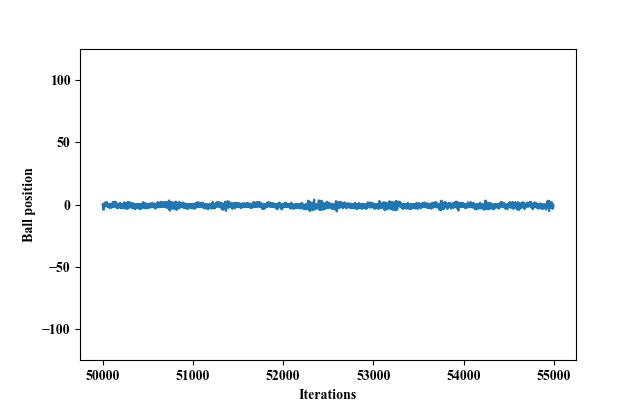
\includegraphics{100_small}
	\caption{The position of the ball over 5000 actions. Note that the width of the tray is 125 in each direction, so the ball stays very confortably in the centre}
\end{figure}
\begin{figure}[H]
	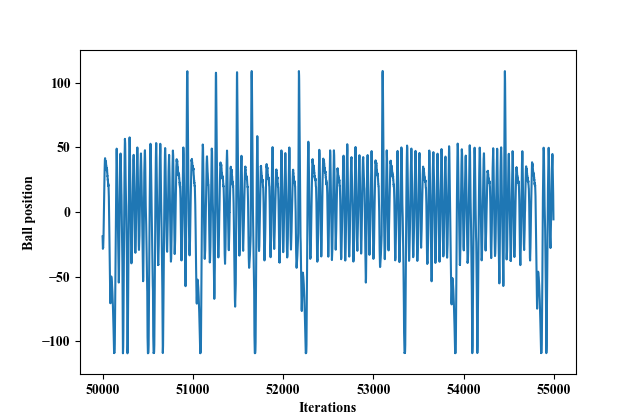
\includegraphics{101_small}
	\caption{An example of learnt behaviour that was not successful. The initial eploration rate was 0.2, reduction value was 1.5, number of reductions was 5. The repetition of the pattern shows that it has slightly learnt the ability to balance, however the amplitude is large. The ball also goes to the end quite frequently}
\end{figure}
%Sims 88 to 115 compares exploration rate stuff
% After 1st round of tests, 100 was best. This is erv:1.5, init:0.5, num:20. About 30000 iterations to converge
%\subsubsection{Initial exploration rate}

Learn rate and discount factor were also experimented using the same method. Low values of both gave poor results, and for the higher values, difference in performance was relatively small. However throguh repreated tests it was found that the best values were a learn rate of 0.4 and a discount factor of 0.9. These results make sense. The learn rate is just below half, showing that the new information is important to the updating process, but is just a bit less important than the existing data. Anything higher could drown out the existing value stored, and since there is quite a lot of exploration, especially early on, it is important to not let the agent change its values too hastily. The discount factor is high since for a task like this it is certainly important to value future actions. If not, it would send the ball to the centre of the tray as quick as possible, whether sometimes it is better to move it gradually to avoid overshooting. A possible reason 0.9 was superior to 0.99 (if only marginally) is that it is sometimes important to focus on the very short term, for instance when right at the edge of the tray - it is better to move the ball away quickly than roll off.

Convergence speed is another important aspect to learning. In a small task like this training takes less than a minute. For a larger task however, it is important to reach the desired performance level as soon as possible. It is hard to know when the task is fully leant since there is no exact completion criteria. However, looking at the plot of position against time for the whole learning procedure can show when the ball is kept in a constant position. Figure 2 shows this for the agent learning over 50000 iterations with the refined parameters.
\begin{figure}[H]
	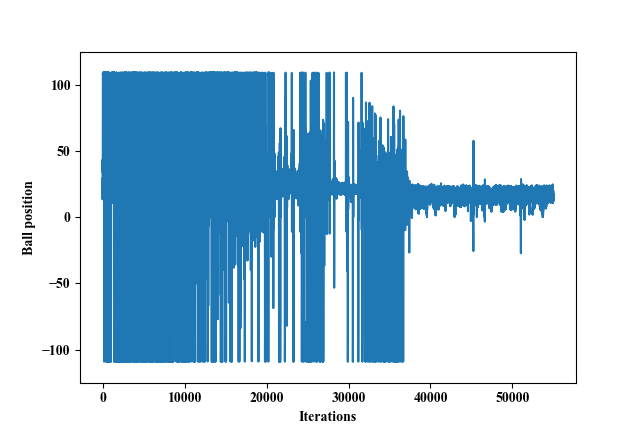
\includegraphics{153_small}
	\caption{The position of the ball over an entire training session. At the start the ball rapidly rolls between weither side of the tray. Over time this becomes less frequent as behaviour to prevent this is leanrt, and the random actions happen less frequently. By the end of the training, the ball is kep consistenyl in the middle of the tray.}
\end{figure}
Figure 3 shows that convergence happens at about 30000 time steps. The training was re-run with the number of iterations as 30000. Figure 4 shows the output. As can be seen, the perfornace was not good and the system did not learn. This is most likely because the exploration rate is linked to the number of iterations, so the reduction of exploration rate will happen faster if there are fewer iterations. Plus, 30000 was only just when the agent learnt the bahaviour, learning still continued past this and solidified the behaviour.
\begin{figure}[H]
	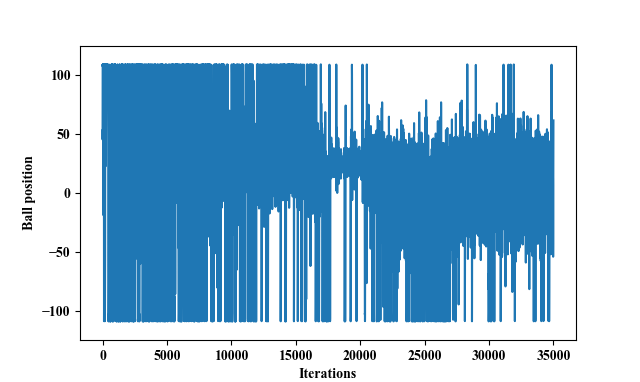
\includegraphics{154_small}
	\caption{The position of the ball over a shorter training session. Performance was worse and the agent did not get a chance to learn the correct behaviour. The x axis goes up to 35000 because of the extra 5000 iterations that do not involve learning.}
\end{figure}
\begin{table}[htb]
\centering
\caption{FINAL Q-LEARNING PARAMETERS}
\vspace*{6pt}
\label{q_params}
\begin{tabular}{>{\raggedright}p{0.4\linewidth}p{0.2\linewidth}}\hline
Parameter & Refined Value\\ \hline\hline
Initial exploration rate & 0.5\\ \hline
Exploration rate reduction frequency & 20\\ \hline
Exploration rate reduction value & 33.3\% \\\hline
Learn rate & 0.4 \\\hline
Discount factor & 0.9 \\\hline
\end{tabular}
\end{table}


\subsection{Specific Reward Q-learning in Simulation}
SHOW HOW IT POERFORMS IN SIMULATION
\subsection{General Reward Q-learning in Simulation}
SHOW HOW IT POERFORMS IN SIMULATION
\subsection{Specific Reward Q-learning with Robot}
\subsection{General Reward Q-learning with Robot}
\subsection{Refined Q-learning in Simulation}
\subsection{Refined Q-learning with Robot}
\section{Evaluation}
\section{Conclusion}


\bibliography{projectpaper}


\end{document}